\documentclass[tikz,border=7pt]{standalone}
\usetikzlibrary{automata,positioning,arrows.meta}
\begin{document}
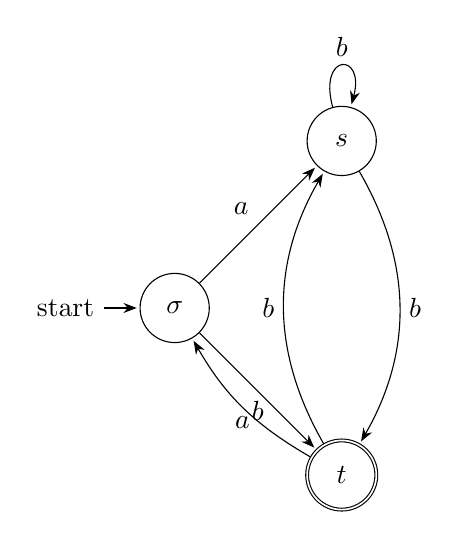
\begin{tikzpicture}[>=Stealth,shorten >=1pt,node distance=3cm,on grid,auto]
\node[state,initial] (q) {$\sigma$}; \node[state] (s) [above right=of q] {$s$}; \node[state,accepting] (t) [below right=of q] {$t$};
\path[->] (q) edge node {$a$} (s) edge node[below] {$b$} (t)
 (s) edge[loop above] node {$b$} () edge[bend left] node {$b$} (t)
 (t) edge[bend left] node {$b$} (s) edge[bend left=15] node[below] {$a$} (q);
\end{tikzpicture}
\end{document}
